\documentclass[12pt]{article}
\usepackage{ctex}%引入中文字符的包
\usepackage{enumerate}%引用标号需要引入的包
%\usepackage{array}
\usepackage{graphicx}%用来在文档中插入图片
\usepackage{caption}%修改图注相关
\usepackage{subfigure}%用来插入并列的图片
\usepackage{float}%确定图片是否为浮动,而不是在一个固定的地方
\usepackage[a4paper,left=31.8mm,right=31.8mm,top=25.4mm,bottom=25.4mm]{geometry}
\begin{document} 
\begin{titlepage}
\begin{center}      
{\Huge \bfseries 机器学习实验报告}\\[1cm]
{\Large \bfseries 多项式拟合正弦曲线}\\[10cm]
{\Large 姓名:秦海滨}\\[1cm]
{\Large 学号:1180300523}\\[8cm]
{\Large 2020年10月6号}
\end{center}
\end{titlepage}
\newpage
\tableofcontents
\newpage
\section{实验目的}
掌握最小二乘法求解(无惩罚项的损失函数)、掌握加惩罚项(2范数)的损失函数优化、梯度下降法、共轭梯度法、理解过拟合、克服过拟合的方法(如加惩罚项、增加样本)。
\section{实验要求及环境}
\subsection{实验要求}
\noindent 1. 生成数据,加入噪声;\par
\noindent 2. 用高阶多项式函数拟合曲线;\par
\noindent 3. 用解析解求解两种loss的最优解(无正则项和有正则项);\par
\noindent 4. 优化方法求解最优解(梯度下降,共轭梯度);\par
\noindent 5. 用你得到的实验数据,解释过拟合;\par
\noindent6. 用不同数据量,不同超参数,不同的多项式阶数,比较实验效果;\par
\noindent7. 语言不限,可以用matlab,python。求解解析解时可以利用现成的矩阵求逆。梯度下降,共轭梯度要求自己求梯度,迭代优化自己写。不许用现成的平台,例如pytorch,tensorflow的自动微分工具。\par
\subsection{实验环境}
\noindent 操作系统:Windows10 \par
\noindent 开发环境:Spider 4.1.4,Python 3.8 \par
\section{数学原理简介}
根据高等数学中学习的泰勒级数的概念,任何的函数都可以被足够高阶的多项式所拟合。在本次实验中就要求我们通过多项式以及各类优化方式去拟合正弦函数$\sin (2 \pi x)$,在m次多项式中,有m+1个待定系数,我们记系数由低到高组成的列向量为$w$。为了确定更加精确的$w$,我们可以使用最小二乘法、加入惩罚项的优化、梯度下降法、共轭梯度法等方式对求解过程进行优化,克服拟合过程中的过拟合问题,以达到更精准的拟合结果。\par
\section{数据的产生}
在此,我们给定产生的原始数据的个数N,在区间$(0,1)$上均匀产生N个数据点,其中噪声noise通过一个正态函数产生,其均值$\mu$和方差$\sigma$可由用户自定义输入,根据$y=sin(2\pi x)+noise$产生所有的数据。在生成所有的数据点后,利用循环将数据转换为矩阵形式即可。\par
\section{最小二乘法拟合(无惩罚项的损失函数)}
在此要求我们用不带惩罚项的解析解方式求出使损失函数达到最小值的系数向量$w$,误差函数的定义如下:
\[E(w)=\frac{1}{2}\sum_{i=1}^{N}({y(x_i,w)-y_i})^2\]\par
将上式写成矩阵形式为:
\[E(w)=\frac{1}{2}(Xw-Y)^T(Xw-Y)\]\par
对上式求导可得:
\[\frac{\partial E}{\partial w}=(X^TX)w-X^TY\]\par
通过令导数为0,我们可以求出极值点,从而求出使损失函数最小的$w$的值,记作$w^*$,解析解为:
\[w^*=(X^TX)^{-1}X^TY\]\par
由此,我们就通过不加惩罚项的解析解方式对数据进行了拟合。\par
在此,我们给出样本数量N为10的时候,最小二乘法在不同的阶数下的拟合情况:\par
\begin{figure}[H]
    \centering
    \subfigure[多项式阶数为2]{
    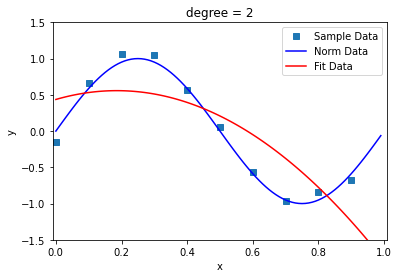
\includegraphics[width=0.45\textwidth]{Fig1.png} 
    }
    \subfigure[多项式阶数为4]{
    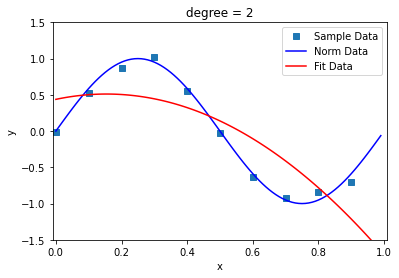
\includegraphics[width=0.45\textwidth]{Fig2.png}
    }
    \subfigure[多项式阶数为8]{
    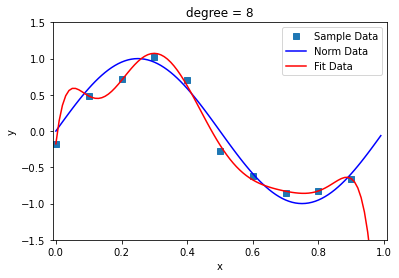
\includegraphics[width=0.45\textwidth]{Fig3.png}
    }
    \subfigure[多项式阶数为16]{
    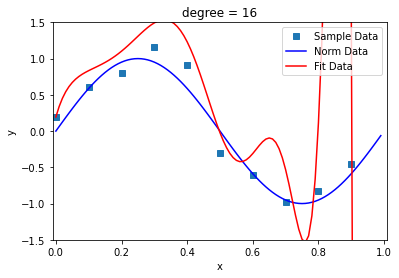
\includegraphics[width=0.45\textwidth]{Fig16.png}
    }
\end{figure}
观察所有的运行结果后,我们发现当多项式阶数较低时,拟合效果并不好,出现了欠拟合现象;当多项式阶数较高时,出现了明显的过拟合现象;仅有多项式阶数为3,4,5的时候,拟合效果良好。
\section{加入惩罚项(2范数)的损失函数优化}
为了解决上一节实验中阶数较高时的过拟合问题,我们可以通过在损失函数式中加入$w$的惩罚项,以解决当参数过多时$w^*$具有较大的绝对值的问题。加入惩罚项后的损失函数式如下:
\[\tilde E(w)=\frac{1}{2}\sum_{i=1}^{N}({y(x_i,w)-y_i})^2+\frac{\lambda}{2}{||w||}^2\]\par
同样,将上式转换为矩阵形式,如下:
\[\tilde E(w)=\frac{1}{2}[(Xw-Y)^T(Xw-Y)+\lambda w^Tw]\]\par
对上式求导可得:
\[\frac{\partial\tilde{E}}{\partial w}=(X^TX)w-X^TY+\lambda w\]\par
令导数为0,我们可以解出$w^*$如下,其中$I$为单位阵:
\[w^*=(X^TX+\lambda I)^{-1}X^TY\]\par
同样控制样本数量为10的情况下,令惩罚项系数$\lambda = 0.0005$加入惩罚项后的拟合结果如下:
\begin{figure}[H]
    \centering
    \subfigure[多项式阶数为2]{
        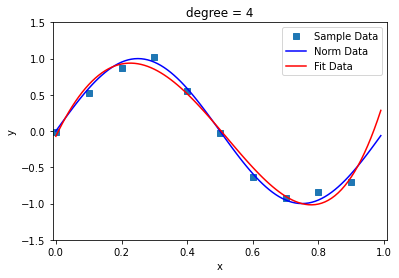
\includegraphics[width=0.45\textwidth]{Fig4.png} 
    }
    \subfigure[多项式阶数为4]{
        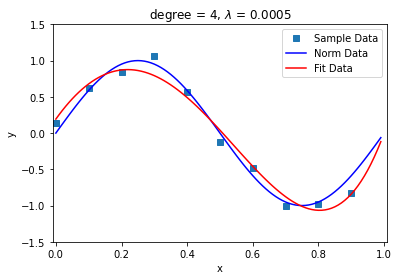
\includegraphics[width=0.45\textwidth]{Fig5.png}
    }
    \subfigure[多项式阶数为8]{
        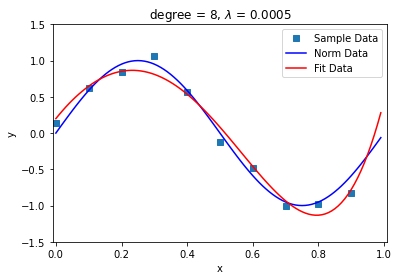
\includegraphics[width=0.45\textwidth]{Fig6.png}
    }
    \subfigure[多项式系数为16]{
        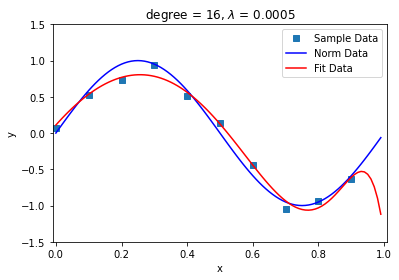
\includegraphics[width=0.45\textwidth]{Fig7.png}
    }
\end{figure}
我们可以明显的观察到,当阶数较低时,欠拟合现象依然存在,但随着阶数的增多,过拟合现象已经得到了有效的控制。在后续的实验验证过程中,我们会发现$\lambda$的大小对于过拟合现象的控制有着很大的影响。$\lambda$很小时,几乎无法抑制过拟合现象,但当$\lambda$过大时,其对于拟合结果的影响又太大,无法做到准确的拟合结果。\par
\section{梯度下降法优化}
对于损失函数$E(w)$,若其在$w_i$点处可微且有定义,我们可以通过其梯度的反方向$-\nabla E(w_i)$调整$w_i$的值,迭代式如下,其中$\eta$为步长,即学习率:
\[w_{i+1}=w_i-\eta\nabla E(w_i)\]\par
在不断的迭代过程中,$w$会逐渐靠近极值点,当达到最大的迭代次数或两次迭代间的差值足够小时停止迭代,此时的$E(w)$为其极小值。\par
同样,我们对加惩罚项的损失函数进行化简求导,结果如下:
\[\frac{\partial{E}}{\partial w}=(X^TX)w-X^TY+\lambda w\]\par
需要注意的是,在迭代过程中,若后一次迭代的损失值比前一次迭代的损失值更大,我们可以通过减少步长以达到更准确的优化结果。\par
在此,我们设置惩罚项系数$\lambda = 0.0001$,最大迭代次数为100000,步长$\eta=0.5$,精确度$\epsilon = 1e-6$,代码运行结果如下:
\begin{figure}[H]
    \centering
    \subfigure[多项式阶数为2]{
        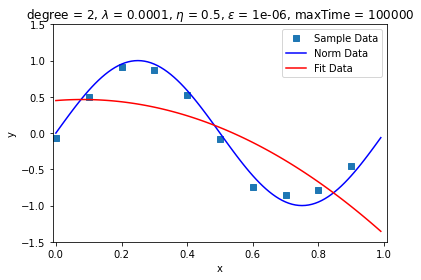
\includegraphics[width=0.45\textwidth]{Fig8.png} 
    }
    \subfigure[多项式阶数为4]{
        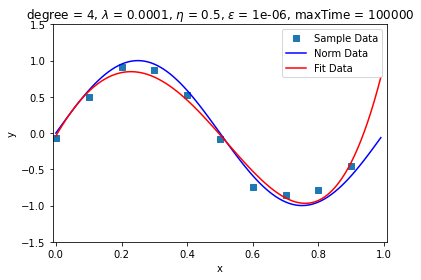
\includegraphics[width=0.45\textwidth]{Fig9.png}
    }
    \subfigure[多项式阶数为8]{
        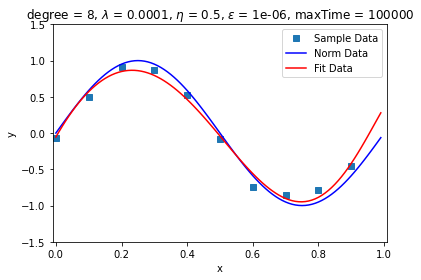
\includegraphics[width=0.45\textwidth]{Fig10.png}
    }
    \subfigure[多项式系数为16]{
        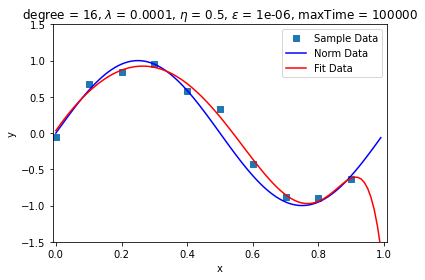
\includegraphics[width=0.45\textwidth]{Fig11.png}
    }
\end{figure}
梯度下降法能够以多次迭代的方式逼近最优解,但在特殊情况下,可能会陷入局部最优解中而无法取得最优解。且在这种迭代方式下,由于求出的解会无限趋近于最优解但由于迭代次数以及精度限制很难达到最优解,所以不会出现明显的过拟合现象。
\section{共轭梯度法优化}
在前两种拟合方法,即带正则和不带正则的解析解方法中,都涉及到一个十分困难的问题,即矩阵求逆。矩阵求逆在计算机中的代价是十分巨大的,共轭梯度法的提出,让我们能够通过迭代的方式求解问题,而不必对系数矩阵求逆。并且,在梯度下降法中,可能会经过很多次的迭代才能得出最终的结果,其消耗的时间十分漫长,每次梯度下降的方向都与上次正交。那么这就为我们留出了一定的优化空间,假设我们选取一组线性无关的方向向量$\{d_0,d_1,\dots,d_n\}$,保证在每一个方向上只下降一次,这样就能避免重复的下降以达到最快的逼近目的。\par
共轭梯度法是一个典型的共轭方向法,它的每一个搜索方向是相互共轭的,而这些搜索方向仅仅是负梯度方向与上一次迭代的搜索方向的组合,因此,存储量少,计算方便。\par
在共轭梯度法中,令下列导数为0:
\[\frac{\partial{E}}{\partial w}=(X^TX)w-X^TY+\lambda w\]\par
此时问题转换为求下式的解析解:
\[(X^TX+\lambda)w=X^TY\]\par
记$Q=X^TX+\lambda,b=X^TY$,该方程的解转换为求$min_{w\in R^n}\frac{1}{2}w^TQw-b^Tw$,之后我们就可以根据迭代式进行m+1次迭代,求解出最终的拟合结果,迭代式如下,初始状态下$p_0=r_0$:
\[w_{i+1}=w_i+\alpha_kp_k\]
\[r_{k+1}=r_k-\alpha_kQp_k\]
\[p_{k+1}=r_{k+1}+\beta_{k+1}p_k\]
\[\alpha_k=\frac{p_k^Tr_k}{p_k^TQp_k}\]
\[\beta_{k+1}=\frac{r_{k+1}^Tr_{k+1}}{r_k^Tr_k}\]\par
我们取惩罚项系数$\lambda=0.0005$,精确度$\epsilon=1e-5$,使用共轭梯度法的拟合结果如下:
\begin{figure}[H]
    \centering
    \subfigure[多项式阶数为2]{
        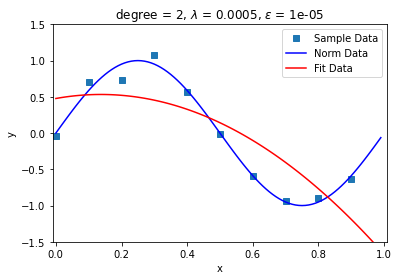
\includegraphics[width=0.45\textwidth]{Fig12.png} 
    }
    \subfigure[多项式阶数为4]{
        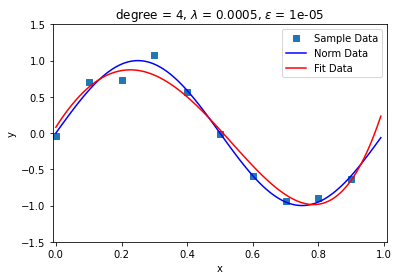
\includegraphics[width=0.45\textwidth]{Fig13.png}
    }
    \subfigure[多项式阶数为8]{
        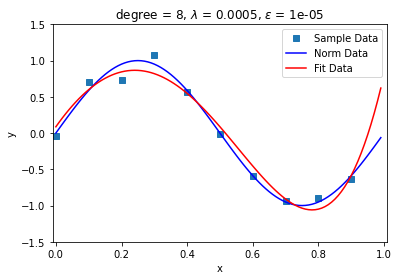
\includegraphics[width=0.45\textwidth]{Fig14.png}
    }
    \subfigure[多项式系数为16]{
        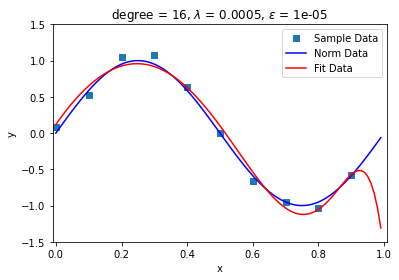
\includegraphics[width=0.45\textwidth]{Fig15.png}
    }
\end{figure}
我们可以明显的观察到,在代码运行过程中,共轭梯度法的拟合速度相比较于梯度下降法加快了许多。与梯度下降法类似的,共轭梯度法的拟合结果也没有明显的过拟合现象。
\section{总结}
通过以上多种方法的实验,我们基本完成了所有的实验内容,可以通过以上的实验数据进行进一步的总结和分析,下面分几个小节进行总结。
\subsection{多项式阶数对于模型的影响}
在不加惩罚项的最小二乘法拟合过程中,我们可以明显地观察到随之多项式次数的增多,明显发生了过拟合现象,我们设置了训练集用于拟合曲线,设置测试集用于检验最终模型的泛化能力,得出的结果如下:
\begin{figure}[H]
    \centering
    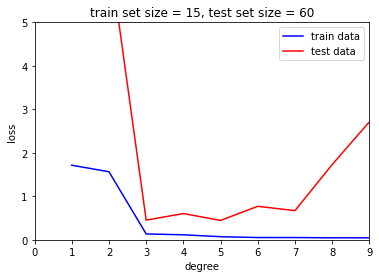
\includegraphics[width=0.7\textwidth]{s1.png}
\end{figure}
我们可以明显地观察到,当多项式阶数较低时,模型的在训练集和测试集上的效果都不理想,损失较大;当多项式在七阶以上时,又出现了过拟合现象,模型对于训练集的拟合程度较为优异,损失持续下降,但对于测试集的数据测试结果会变的不受控制,损失逐渐上升。这就是因为多项式阶数的上升引起的过拟合现象影响了模型的拟合能力。随着阶数的上升,模型的表达能力上升,模型对于训练集中的数据的的表示越来越准确,但为了准确表示这些数据,$w^*$中的某些系数会变得很大,这不利于模型描述训练集之外的数据,即降低了模型的泛化能力。\par
\subsection{超参数$\lambda$对于模型的影响}
为了解决当多项式阶数增加时的过拟合现象,我们修改了损失函数表达式,添加了惩罚项以控制$w^*$中个别项的系数绝对值过大的问题,其中惩罚项的系数$\lambda$的大小对于模型有着较大的影响,实验结果如下:
\begin{figure}[H]
    \centering
    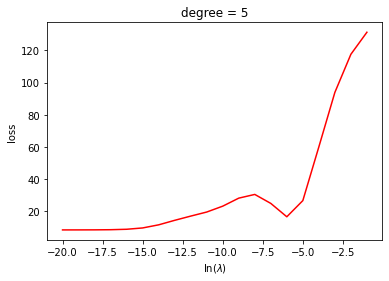
\includegraphics[width=0.7\textwidth]{s2.png}
\end{figure}
从实验结果,我们可以观察到,当惩罚项系数$\lambda$过小时,相当于没有惩罚项;随着$\lambda$的增大,loss逐渐减小,但当$\lambda$再变大的时候,其对整个模型的影响效果就变得十分严重,loss会由于$\lambda$的增大迅速升高。这就要求我们在模型建立的过程中找到一个合适的惩罚项系数以达到优化模型的目的。
\subsection{训练集数据量对于模型的影响}
显然,训练集中的数据量对于模型有着较大的影响,我们改变训练集的大小,可以观察到在一定阶数下的模型的拟合能力的变化,如下:
\begin{figure}[H]
    \centering
    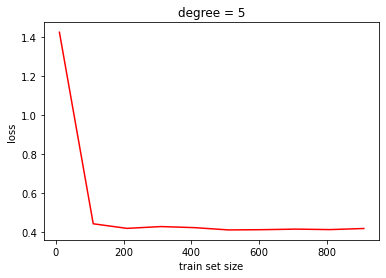
\includegraphics[width=0.7\textwidth]{s3.png}
\end{figure}
由图可知,在多项的阶数一定时,不断扩充训练集的大小,会持续提高模型的拟合能力,降低损失。由于数据的大量增加,噪声的影响会逐渐减小,模型能通过更多的数据改进自己的能力,使自己更加准确,泛化能力更强,有效改善过拟合现象。\par
\subsection{为什么会发生过拟合?}
根据所有的实验数据,我认为是由于训练集中的数据有限且不足,并且由于加入的噪声影响,在阶数不断上升的过程中,模型对于训练集中的数据的表达能力不断加强,能够十分准确的表达训练集中的数据,并且为了达到这个目的,使$w^*$的中的部分系数绝对值非常大,导致该模型虽然能够准确的表达训练集的内容,但却失去了其应该有的泛化能力,不利于整个模型的拟合结果,因此出现了过拟合现象。我们可以通过加入惩罚项或者增加数据量的方式改善过拟合现象。
\subsection{结论}
在本次实验中,我们通过了多种方法实现并优化了多项式拟合正弦曲线。讨论了多种因素对于模型的影响。首先,模型的复杂度于模型的参数个数(多项式阶数)以及模型的参数$w^*$的绝对值(范数)有关,模型过于简单(阶数较低)会出现欠拟合现象,而模型过于复杂(阶数较高),会出现过拟合现象。特别在模型复杂时,$w^*$往往具有较大的绝对值,这会直接导致模型的泛化能力减弱,对其拟合效果有着不好的影响。\par
我们可以通过增加惩罚项的方式改善阶数较高时的过拟合问题,通过惩罚项降低参数的绝对值,使模型复杂度与问题匹配。当惩罚项较大时,会导致模型出现欠拟合问题;当惩罚项较小时,又无法有效改善过拟合问题。我们可以将数据集分为训练集、验证集和测试集来调试$\lambda$的值。\par
除此之外,数据量的多少对于模型的建立也有着重要的影响,模型能够在更大的数据量中改进自己的能力以达到更好的拟合效果。\par
此外,在梯度下降法中,需要注意我们需要根据实验数据的实际情况改变下降步长,即在后一次迭代的效果不如前一次迭代时,我们就需要减少步长以达到更好的优化目的。\par
\end{document}